% Drawing 74/03-3 -- folder 74, batch 03, archive page 43 (PDF page 44).
% Transcription: dans la moitié inférieure, un grand diagramme de flèches entre les ensembles « (tria$'$) », « Hex », « Tritria », « (tria) $\times$ hex », « (tria $\times$ 2) $\times$ hex $+$ \ill{} », « hex $+$ diag », « hex $+$ sommets », « Hexorien $\simeq$ (tria$'$/Hex) », « (trilles) $= \tau\times\varepsilon\times\omega(\tau)$ », $S$, $R \rightrightarrows \tau\times\varepsilon,\ \tau\times\varepsilon'$, les flèches portant les degrés $2$ ou $3$ ; en bas, un hexagone avec ses diagonales.
% Kind: arrow diagram between named sets (coverings), with a hexagon. Method 2 (schematic redraw from the facsimile). Status: partial.
% Notes: The labels are placed where they stand and joined by the arrows as seen; the degrees 2 and 3 are put by the arrows they stand beside. Struck words are drawn grey. The direction of a few arrows and some labels (« (tri) » in the middle row, the struck block under R) are uncertain. Bottom right: a hexagon with its diagonals (overinked, drawn schematically).
% Coordinates: 1 unit = 1 mm = 1/100 of the crop width (bbox in page fractions: [0.05, 0.45, 0.95, 0.93]).
% Redrawn by Claude (claude-opus-5-5), issue #73, 2026-11-07; not checked by a human; not compiled (no TeX in the session).
% Rights: reproduces part of the work -- behind RENDER_TRANSCRIPTS, never published by itself.
\documentclass[tikz,border=3pt]{standalone}
\usepackage{amsmath,amssymb}
\usetikzlibrary{patterns,arrows.meta}
\tikzset{pencil/.style={black!45}, struck/.style={black!35}, mark/.style={circle,draw,inner sep=1.3pt}, pt/.style={circle,fill,inner sep=0.9pt}, opt/.style={circle,draw,fill=white,inner sep=1.1pt}}
\begin{document}
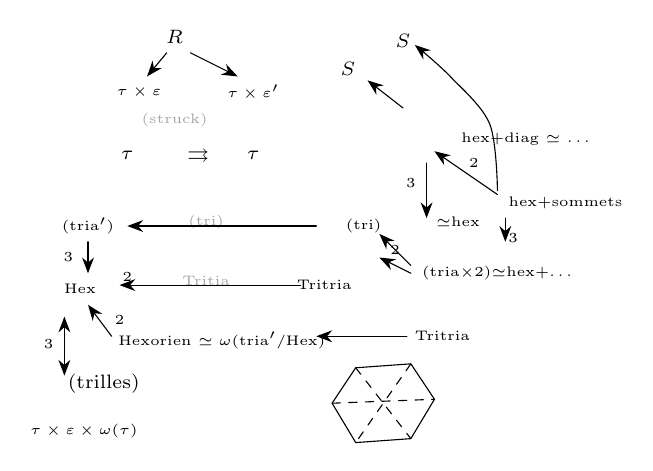
\begin{tikzpicture}[x=1mm,y=1mm,line cap=round,line join=round,font=\scriptsize]
\node[inner sep=1pt] at (38,-7) {\scriptsize $R$};
\draw[-{Stealth[length=2mm]}] (37,-9) -- (34.5,-12);
\draw[-{Stealth[length=2mm]}] (40,-9) -- (46,-12);
\node[inner sep=1pt] at (33.5,-14) {\tiny $\tau\times\varepsilon$};
\node[inner sep=1pt] at (48,-14) {\tiny $\tau\times\varepsilon'$};
\node[inner sep=1pt,struck] at (38,-17.5) {\tiny (struck)};
\node[inner sep=1pt] at (32,-22) {\scriptsize $\tau$};
\node[inner sep=1pt] at (41,-22) {\scriptsize $\rightrightarrows$};
\node[inner sep=1pt] at (48,-22) {\scriptsize $\tau$};
\node[inner sep=1pt] at (60,-11) {\scriptsize $S$};
\draw[-{Stealth[length=2mm]}] (67,-16) -- (62.5,-12.5);
\node[inner sep=1pt] at (67,-7.5) {\scriptsize $S$};
\draw[-{Stealth[length=2mm]}] plot[smooth, tension=0.55] coordinates {(79,-26.5) (78,-18) (73,-12) (68.5,-8)};
\node[inner sep=1pt,anchor=west] at (74,-20) {\tiny hex$+$diag $\simeq$ \dots};
\node[inner sep=1pt,anchor=west] at (80,-28) {\tiny hex$+$sommets};
\draw[-{Stealth[length=2mm]}] (79,-27) -- (71,-21.5);
\node[inner sep=1pt] at (76,-23) {\tiny $2$};
\draw[-{Stealth[length=2mm]}] (70,-23) -- (70,-30);
\node[inner sep=1pt] at (68,-25.5) {\tiny $3$};
\node[inner sep=1pt] at (74,-30.5) {\tiny $\simeq$hex};
\draw[-{Stealth[length=2mm]}] (80,-30) -- (80,-33);
\node[inner sep=1pt] at (81,-32.5) {\tiny $3$};
\node[inner sep=1pt] at (27,-31) {\tiny (tria$'$)};
\node[inner sep=1pt,struck] at (42,-30.5) {\tiny (tri)};
\node[inner sep=1pt] at (62,-31) {\tiny (tri)};
\draw[-{Stealth[length=2mm]}] (56,-31) -- (32,-31);
\draw[-{Stealth[length=2mm]}] (27,-33) -- (27,-37);
\node[inner sep=1pt] at (24.5,-35) {\tiny $3$};
\node[inner sep=1pt] at (26,-39) {\tiny Hex};
\node[inner sep=1pt] at (57,-38.5) {\tiny Tritria};
\draw[-{Stealth[length=2mm]}] (54,-38.5) -- (31,-38.5);
\node[inner sep=1pt] at (32,-37.5) {\tiny $2$};
\node[inner sep=1pt,struck] at (42,-38) {\tiny Tritia};
\node[inner sep=1pt,anchor=west] at (69,-37) {\tiny (tria$\times$2)$\simeq$hex$+$\dots};
\draw[-{Stealth[length=2mm]}] (68,-36) -- (64,-32);
\node[inner sep=1pt] at (66,-34) {\tiny $2$};
\draw[-{Stealth[length=2mm]}] (68,-37) -- (64,-35);
\node[inner sep=1pt] at (44,-45.5) {\tiny Hexorien $\simeq\omega$(tria$'$/Hex)};
\draw[-{Stealth[length=2mm]}] (30,-45) -- (27,-41);
\node[inner sep=1pt] at (31,-43) {\tiny $2$};
\node[inner sep=1pt] at (72,-45) {\tiny Tritria};
\draw[-{Stealth[length=2mm]}] (67.5,-45) -- (56,-45);
\draw[{Stealth[length=2mm]}-{Stealth[length=2mm]}] (24,-42.5) -- (24,-50);
\node[inner sep=1pt] at (22,-46) {\tiny $3$};
\node[inner sep=1pt] at (29,-51) {\scriptsize (trilles)};
\node[inner sep=1pt] at (26.5,-57) {\tiny $\tau\times\varepsilon\times\omega(\tau)$};
\draw (61,-49) -- (68,-48.5) -- (71,-53) -- (68,-58) -- (61,-58.5) -- (58,-53.5) -- cycle;
\draw[dashed] (61,-49) -- (68,-58);
\draw[dashed] (68,-48.5) -- (61,-58.5);
\draw[dashed] (58,-53.5) -- (71,-53);
\end{tikzpicture}
\end{document}
